\chapter{Resultados}
\label{cap:resultados}

Neste Capítulo são descritos os resultados obtidos da execução dos testes descritos no capítulo anterior. Para cada ambiente de teste, o agente foi treinado uma vez utilizando o módulo de motivação intrínseca e uma vez sem utilizá-lo pelo mesmo número de iterações. Na análise, nos referimos ao agente do segundo treinamento como algoritmo, ou agente, \textit{baseline}. Dizemos também que o algoritmo "convergiu" quando sua razão de sucessos se torna satisfatória. Em todos os gráficos, o eixo horizontal representa o número de iterações, as linhas em vermelho indicam o uso do algoritmo PPO com motivação intrínseca, ou curiosidade, e as linhas azuis indicam o uso algoritmo PPO \textit{baseline}. Nos gráficos de recompensa intrínseca e de divergência KL as linhas foram suavizadas\footnote{O filtro de Savitzky-Golay, implementado pela biblioteca SciPy \cite{scipy}, foi utilizado com uma janela de tamanho 31 e ordem polinomial 3.} para melhor compreensão. Os resultados foram agrupados de acordo com os ambientes treinados e uma análise geral é feita ao final deste Capítulo.

% - - - - - - - - - - - - - - - - - - - - - - - - - - - - - - - - - - -
\section{\textit{FetchReach}}
\label{sec:reach}

\begin{figure}[h!]
 \centering
  \subfigure[Início do episódio.]
   {
    \includegraphics[width=0.3\textwidth]{./fig/reach_ex_1}
    \label{subfig:reach_ex_1}
   }
  \subfigure[Episódio em progresso.]
   {
    \includegraphics[width=0.3\textwidth]{./fig/reach_ex_2}
    \label{subfig:reach_ex_2}
   }
  \subfigure[Próximo do fim do episódio.]
   {
    \includegraphics[width=0.3\textwidth]{./fig/reach_ex_3}
    \label{subfig:reach_ex_3}
   }
   \captionsetup{width=1\textwidth}
   \caption{Progresso do agente treinado com curiosidade no ambiente FetchReach.}
  \label{fig:reach_ex}
\end{figure}

No ambiente \textit{FetchReach}, ambos os algoritmos alcançaram 100\% de sucesso em menos de dois milhões de passos de simulação. A Figura \ref{fig:reach_ex} mostra o agente treinado com módulo de curiosidade em alguns passos de simulação. É interessante notar o decaimento do valor da recompensa intrínseca (Figura \ref{subfig:reach_int}) em um ritmo semelhante ao aumento da razão de sucessos do algoritmo PPO com módulo de curiosidade (Figura \ref{subfig:reach_suc}). Este fenômeno pode indicar o aprendizado da dinâmica do ambiente por parte do agente, ou seja, a medida em que o agente descobre como suas ações influenciam o ambiente e, consequentemente, mais próximo está de seu objetivo, menos surpreso com os novos estados ele fica.

\begin{figure}[h!]
 \centering
  \subfigure[Razão de sucessos.]
   {
    \includegraphics[width=0.45\textwidth]{./fig/reach}
    \label{subfig:reach_suc}
   }
  \subfigure[Recompensa intrínseca média.]
   {
    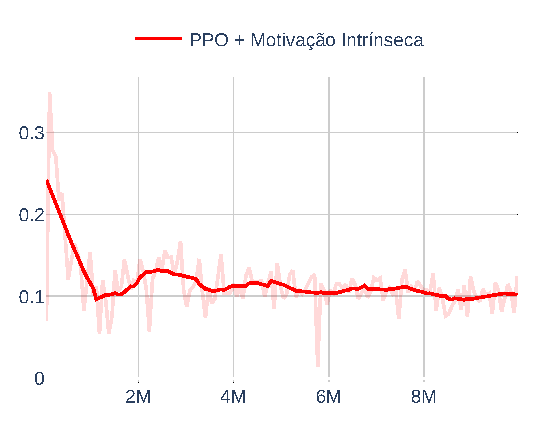
\includegraphics[width=0.45\textwidth]{./fig/reach_int}
    \label{subfig:reach_int}
   }
  \subfigure[Entropia da política.]
   {
    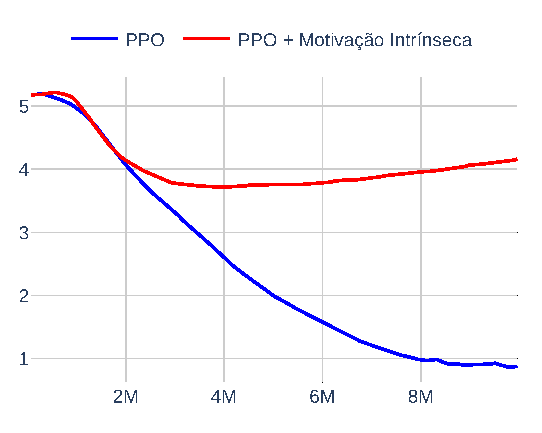
\includegraphics[width=0.45\textwidth]{./fig/reach_ent}
    \label{subfig:reach_ent}
   }
  \subfigure[Divergência KL entre as políticas.]
   {
    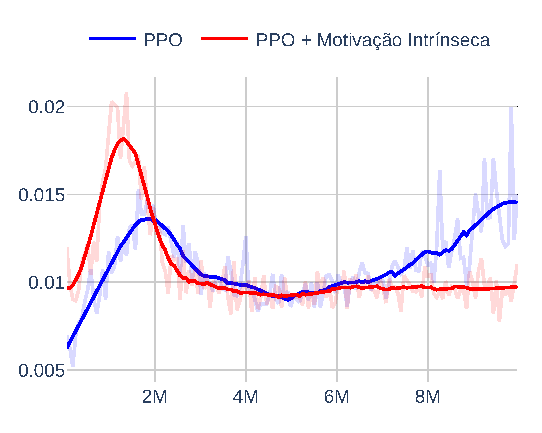
\includegraphics[width=0.45\textwidth]{./fig/reach_kl}
    \label{subfig:reach_kl}
   }
   \caption{Estatísticas para o ambiente FetchReach.}
  \label{fig:reach}
\end{figure}


Outra análise que pode ser feita neste ambiente é em relação aos gráficos de entropia (Figura \ref{subfig:reach_ent}) e divergência KL (Figura \ref{subfig:reach_kl}). A entropia da política do agente com módulo de curiosidade tende a se manter alta mesmo após a convergência do algoritmo, enquanto que o agente \textit{baseline} diminui sua entropia se tornando cada vez mais determinístico. Na prática, vemos que o agente com curiosidade se mantém com altos níveis de exploração, possibilitando que melhores sequências de ações para alcançar o objetivo proposto sejam encontradas. Pode-se observar também pelo gráfico de divergência KL que após a convergência a política do agente com curiosidade tende sofrer poucas modificações em relação à política do agente \textit{baseline}. Este comportamento reforça ainda mais a hipótese de que a dinâmica do ambiente foi aprendida pelo agente com curiosidade, fazendo com que a recompensa intrínseca seja muito menor e as alterações na política sejam mínimas.

% - - - - - - - - - - - - - - - - - - - - - - - - - - - - - - - - - - -

\section{\textit{FetchPush}}
\label{sec:push}

No ambiente \textit{FetchPush} o algoritmo PPO original não conseguiu resolver a tarefa durante o treinamento, como mostra o gráfico da Figura \ref{subfig:push_suc}. Uma explicação é a quantidade de ações em sequência necessárias para alcançar o objetivo, tornando baixa a chance disso ocorrer por acaso. O PPO com módulo de curiosidade, no entanto, pode aproveitar o incentivo que recebe ao explorar as posições do próprio manipulador e, o mais impactante, o comportamento do bloco quando o atinge por acaso. Como a posição, rotação e velocidades do bloco fazem parte da observação do agente e o modelo de futuro não conhece a dinâmica do bloco no início do treinamento, esbarrar no mesmo faz com que o erro de predição aumente de forma significativa. Como o erro de predição é diretamente proporcional à recompensa intrínseca do agente, este se torna consideravelmente interessado em jogar o bloco de um lado para o outro, eventualmente alcançando o objetivo. Quando este processo ocorre, observa-se um pico no gráfico de recompensa intrínseca (Figura \ref{subfig:push_int}) e logo em seguida um aumento na taxa de sucesso (Figura \ref{subfig:push_suc}).

\begin{figure}[h!]
 \centering
  \subfigure[Início do episódio.]
   {
    \includegraphics[width=0.3\textwidth]{./fig/push_ex_1}
    \label{subfig:push_ex_1}
   }
  \subfigure[Episódio em progresso.]
   {
    \includegraphics[width=0.3\textwidth]{./fig/push_ex_2}
    \label{subfig:push_ex_2}
   }
  \subfigure[Fim do episódio.]
   {
    \includegraphics[width=0.3\textwidth]{./fig/push_ex_3}
    \label{subfig:push_ex_3}
   }
   \caption{Progresso do agente treinado com curiosidade no ambiente FetchPush.}
  \label{fig:push_ex}
\end{figure}

\begin{figure}[h!]
 \centering
  \subfigure[Razão de sucessos.]
   {
    \includegraphics[width=0.45\textwidth]{./fig/push}
    \label{subfig:push_suc}
   }
  \subfigure[Recompensa intrínseca média.]
   {
    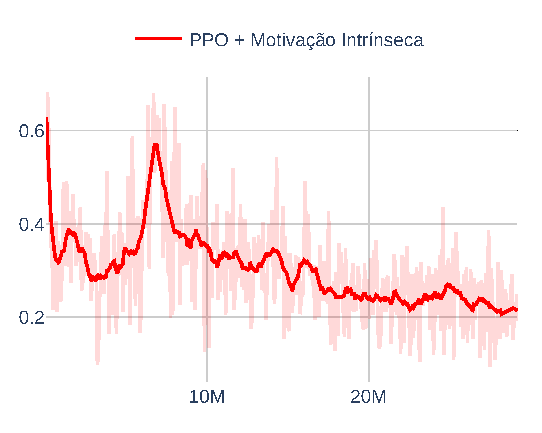
\includegraphics[width=0.45\textwidth]{./fig/push_int}
    \label{subfig:push_int}
   }
  \subfigure[Entropia da política.]
   {
    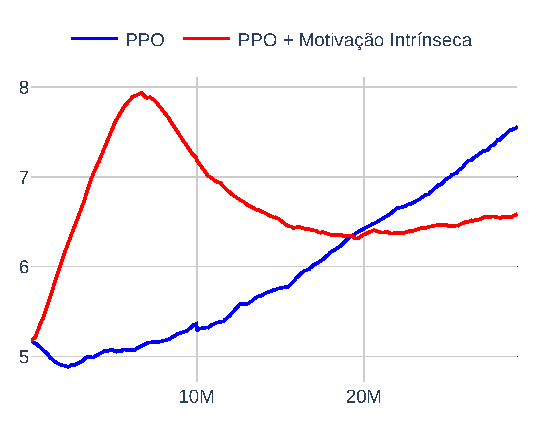
\includegraphics[width=0.45\textwidth]{./fig/push_ent}
    \label{subfig:push_ent}
   }
  \subfigure[Divergência KL entre as políticas.]
   {
    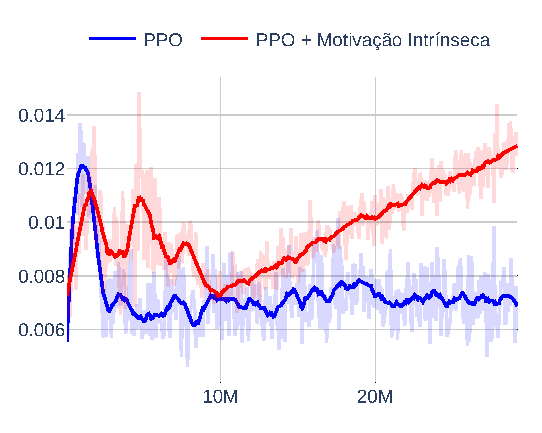
\includegraphics[width=0.45\textwidth]{./fig/push_kl}
    \label{subfig:push_kl}
   }
   \caption{Estatísticas para o ambiente FetchPush.}
  \label{fig:push}
\end{figure}

O gráfico de divergência KL (Figura \ref{subfig:push_kl}) mostra como a política do agente com curiosidade é modificada gradativamente durante o treino, mesmo após a convergência. Como a razão de sucessos ao final do treinamento foi de 96\%, como mostra a Tabela \ref{tab:taxasuc}, e a recompensa intrínseca possuía um valor considerável, acredita-se que o agente poderia melhorar sua política ainda mais. Além disso, o gráfico da Figura \ref{subfig:push_ent} mostra como a entropia da política do agente com curiosidade possui um pico logo no início do treinamento, possivelmente motivado pela recompensa intrínseca, e como a mesma se estabiliza em valores altos após a convergência. O agente \textit{baseline}, por outro lado, não recebendo sinais de como modificar sua política opta por aumentar a entropia das distribuições das ações, reforçando seu comportamento exploratório. Além disso, é possível ver que a divergência KL entre as políticas do agente \textit{baseline} se mantém relativamente constante. Um exemplo de episódio em que o agente treinado com curiosidade consegue resolver a tarefa é mostrado na Figura \ref{fig:push_ex}.

% - - - - - - - - - - - - - - - - - - - - - - - - - - - - - - - - - - -

\section{\textit{FetchPickAndPlace}}
\label{sec:pick}

\begin{figure}[h!]
 \centering
  \subfigure[Início do episódio.]
   {
    \includegraphics[width=0.3\textwidth]{./fig/pick_ex_1}
    \label{subfig:pick_ex_1}
   }
  \subfigure[Episódio em progresso.]
   {
    \includegraphics[width=0.3\textwidth]{./fig/pick_ex_2}
    \label{subfig:pick_ex_2}
   }
  \subfigure[Fim do episódio.]
   {
    \includegraphics[width=0.3\textwidth]{./fig/pick_ex_3}
    \label{subfig:pick_ex_3}
   }
   \captionsetup{width=1\textwidth}
   \caption{Progresso do agente treinado com curiosidade no ambiente FetchPickAndPlace.}
  \label{fig:pick_ex}
\end{figure}

Neste ambiente, assim como em \textit{FetchPush}, o algoritmo PPO original não é capaz de realizar a tarefa durante o treinamento (Figura \ref{subfig:pick_suc}) pelos mesmos motivos. Neste ambiente o desafio é ainda maior, pois uma grande quantidade de ações extremamente específicas devem ser executadas para alcançar o objetivo. Para o PPO com módulo de curiosidade, porém, a tarefa ainda é factível. O agente é recompensado já em poucas iterações após o início do treino ao interagir com o bloco, sendo encorajado a manipulá-lo uma vez que sua posição, rotação e velocidades fazem parte de sua observação, o que influencia em sua recompensa intrínseca (Figura \ref{subfig:pick_int}). Neste caso nota-se também que sua evolução é um processo mais lento, cerca de 15 milhões de iterações para que o agente alcance mais de 85\% de sucesso.

\begin{figure}[h!]
 \centering
  \subfigure[Razão de sucessos.]
   {
    \includegraphics[width=0.45\textwidth]{./fig/pick}
    \label{subfig:pick_suc}
   }
  \subfigure[Recompensa intrínseca média.]
   {
    \includegraphics[width=0.45\textwidth]{./fig/pick_int}
    \label{subfig:pick_int}
   }
  \subfigure[Entropia da política.]
   {
    \includegraphics[width=0.45\textwidth]{./fig/pick_ent}
    \label{subfig:pick_ent}
   }
  \subfigure[Divergência KL entre as políticas.]
   {
    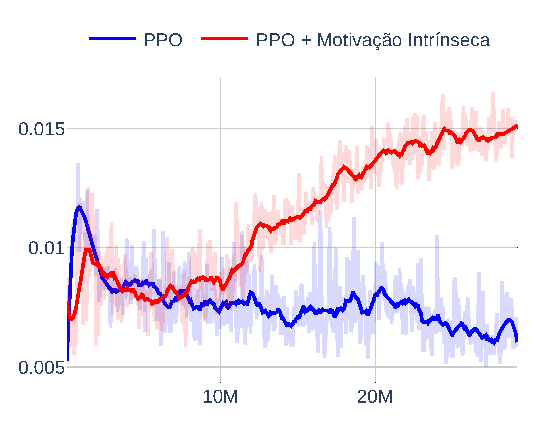
\includegraphics[width=0.45\textwidth]{./fig/pick_kl}
    \label{subfig:pick_kl}
   }
   \caption{Estatísticas para o ambiente FetchPickAndPlace.}
  \label{fig:pick}
\end{figure}

Mais uma vez, há um pico no gráfico de recompensa intrínseca pouco antes da taxa de sucesso do agente começar a subir. A curiosidade do agente diminui poucas iterações após a convergência, uma vez que a dinâmica do ambiente não trás mais tantas novidades. Além disso, observa-se o mesmo comportamento nos gráficos de entropia (Figura \ref{subfig:pick_ent}) e divergência KL entre políticas (Figura \ref{subfig:pick_kl}) se comparado com o ambiente \textit{FetchPush}. O interessante a se notar, porém, é quão conservadora em relação a uniformidade das probabilidades de ações o agente se tornou neste ambiente, como mostra o gráfico de entropia. Esse comportamento é esperado pois o agente deve sempre abrir a garra para segurar o bloco e evitar soltá-lo, uma vez que o mesmo pode cair da mesa, fora de seu alcance. A Figura \ref{fig:pick_ex} mostra o agente treinado com curiosidade resolvendo a tarefa proposta.

% - - - - - - - - - - - - - - - - - - - - - - - - - - - - - - - - - - -

\section{Considerações Gerais}
\label{sec:resgerais}

Em geral, o algoritmo com módulo de curiosidade foi capaz de resolver as tarefas de todos os ambientes, como mostra a Tabela \ref{tab:taxasuc}. É interessante notar que a taxa de sucesso no ambiente \textit{FetchPickAndPlace} é maior que a taxa de sucesso no ambiente \textit{FetchPush}. Isso acontece pois em algumas avaliações no ambiente \textit{FetchPush} o manipulador pode jogar o bloco para fora da mesa, impossibilitando o agente de completar sua tarefa. Em \textit{FetchPickAndPlace} a garra do manipulador robótico raramente solta o bloco uma vez que conseguiu agarrá-lo. Após segurar o bloco, basta que o agente se comporte como em \textit{FetchReach}, o que é uma tarefa simples.

\begin{table*}[h!]
\centering
\captionsetup{width=1\textwidth}
\caption{Razão de sucesso dos algoritmos em cada ambiente de teste.}
\label{tab:taxasuc} 
\begin{tabular}{|c|c|c|c|c|c|c|}
\hline Algoritmo & FetchReach & FetchPush & FetchPickAndPlace \\ 
\hline PPO & 100\% & 0\% & 0\%\\ 
\hline PPO + Motivação Intrínseca & 100\% & 96\% & 99\%\\ 
\hline 
\end{tabular} 
\end{table*}